% -----------------------------------------------------------------------------
%                                Introduction
% -----------------------------------------------------------------------------
\newpage                                                 \chapter{Introduction}
\renewcommand{\thepage }{\arabic{page}}                    \setcounter{page}{1}



%-------------------------- where we're going --------------------------------%

This paper focuses on the roles of audio and notifications within user interface
design. It begins by reviewing findings when audio is used as \textit{the}
primary element of an interface, as explored by~\cite{arons1991hyperspeech,
shilling2000virtual}. Attention is then shifted to the work by Goose et al who
used binaural audio as an interface for HTML presentation
~\cite{goose19993dAudio}. Finally we explore the number of works which have
looked at binaural audio's role  within interfaces incorporating other modals
~\cite{ yu2006novel, marentakis2004study}.

Our research continues with the exploration of the role notifications  have
within interface design. Experiments have shown that the impact of variable
reliability in a notification system biases users to ignore future
notifications~\cite{ leetiernan2001effective}. This paper examines the different
types of notifications: informative ~\cite{maltz2000cue} and interpretted
~\cite{horvitz1999principles}.   We also explore the effective and judicial use
of notification systems to  inform future designs of our work
~\cite{cutrell2001notification}.


%------------------------ Basic Background Info ------------------------------%

Audible interfaces provide an alternate mode of access to computers whenever a
users’ visual focus is unavailable. Visual focus can be unavailable for a number
of reasons, such as when users are driving, using handheld devices while engaged
in other physical activities that command your visual attention, or even as a
result of physical disabilities~\cite{michelis2008disappearing}.

Most audible interfaces only provide a text-to-speech component allowing systems
to read the content of a visual interface to a user.  Text-to-speech solutions
often implement a monoaural speech pattern that provides a user with a single
channel of communication. Techniques exist to provide spatially placed (3D
/ binaural) audio to listeners.



%---------------------- why we're going there --------------------------------%
\section{                  Motivation                                         }

T.V. Raman demonstrated and enumerated the differences between speech output
interfaces and screen reading solutions. He argued that the key difference
was the system's ability to give an application a voice (like Emacspeak) versus
simply reading a screen.  Raman was introducing Emacspeak, an application
intended to give a voice to the terminal, not simply allowing a machine to read
what it is displaying. The precise difference he was making was demonstrating how
creating Emacspeak as a subsystem, it had context specific information available
to it that many screen readers simply cannot duplicate~\cite{raman1996emacspeak}.

To this effect, this project explores positional audio and notification theory
can be combined in multiple ways to create multiple new contexts for user
interface design.  There are four such systems :

\textbf{}

% context aware
% operating system that is able to vocalize each task in a multi-tasking
% environment in a natural manner.

Instead, imagine a world where you had an army of assistants. Furthermore, these
assistants were smart and effective communicators that could succinctly and
politely portray just the right amount of information to you.  You could
orchestrate these assistants any way you'd like, but with the ultimate goal
being to carry conversations with your computational tasks, not have them all
yell at you through disruptive notifications.

Take a common scenario like driving to work on a typical morning. Eric Horvitz
described how intelligent interfaces have been realized, so that the computer
powering the navigation system is also checking current road conditions relative
to your location. Your smartphone has resumed polling your work email address,
your calendar has been updated by a colleague, and your family is messaging you
reminding you of a prior engagement. In his work, he quantified the risks and
benefits of using different notification paradigms to express this information.

If a system existed that conformed to common patterns of communication, audio
would be a major component.  By exploring human psychology and surveying user
preferences, can a system be created that can discern exactly how much or how
little to say when presenting a user with updated information? Can a system be
created that successfully evaluates an individual's preferences and needs,
adjusting settings for both physical constraints such as fine tuning the user
specific head related transfer functions, to the verbosity of given
notifications? By understanding usage patterns for common tasks, such as
navigation, communication the system aims to provide just the right amount of
context for each task a user is performing, creating a framework that minimizes
cognitive load and maximizes productivity.


%-----------------------------------------------------------------------------%
\section{                  Project                                            }


This paper describes a system that supports a new conceptual model that maps
interface elements into a 3D audio space. Using binaural audio as the mechanism,
novel features are discussed that provide information to the user in terms of
spatial attenuation, audio structural survey of content on the web, accurate
positional audio feedback, and an audible progress indicator.  These new
features can improve both the user’s comprehension of content presented to them
while provided with cues to assist recall of information.


Human auditory localization has been studied extensively~\cite{
yost1987directional, blauert1997spatial }. Humans are especially adept at
localizing sounds in three dimensions. Consider a sound source to the left of a
listener.  Sounds from the source arrive at the left ear first, and a short time
after reach the right ear.  The amplitude of the left ear sound will be
attenuated due to head shadowing.


The predominant auditory cues for determining whether a sound is coming from the
left or right directions are the  interaural intensity differences and the
interaural time differences. Humans are also adept at identifying sound position
that are in front of or behind them, along with estimating the sound source's
elevation.  This is possible because the incident sound waves interact with the
torso, head, external ear (pinna) prior to arriving at the inner ear.


The directional dependent filtering to each of a subject's ears can be expressed
as a frequency response, called a head related transfer function (HRTF), and
thus a pair of HRTFs describe how sound from one location reaches the two ears.
HRTFs are usually measured using human subjects or dummy-head microphones which
consist of response pairs for the left an right ears corresponding to a large
number of source positions surrounding the head.


There are two regions of interest when considering source locations of sound.
When the sound is close to the head, the spherical curvature of the incident
sound waves cause the HRTFs to change qualitatively as a function of distance,
but at moderate distances, the incident waves can be considered planar. At
extreme distances, humans are only capable to process auditory cues that only
depend on the sound sources volume.


\begin{figure}[h]
  \centering
  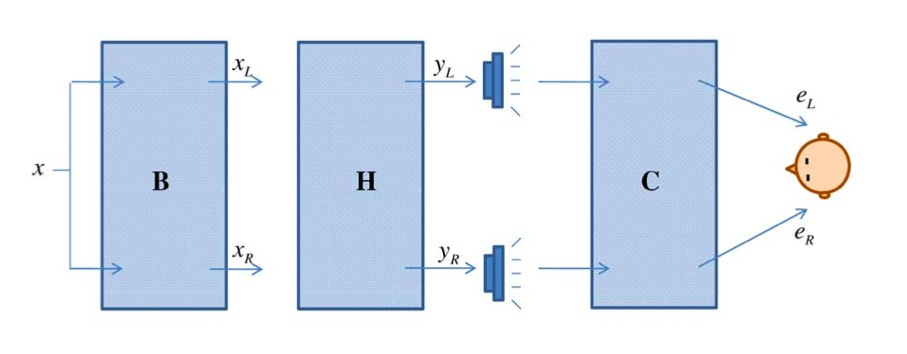
\includegraphics[width=1\textwidth]{images/binaural_diagram.jpg}
  \caption{Schematic of a binaural audio system}
\end{figure}


The remainder of this thesis explores both the questions that remain to be
explored as well as the steps to achieve these goals.


While exploring the research in the utilization of audible interfaces, this
paper works towards two major goals. First a review of the methodologies,
processes, and terms necessary to study audible interfaces is presented. In
conjunction with this, an argument for the benefit of a 3D Audio Interface will
be presented as an accessible solution for users with visual disabilities.

A general background of Binaural Audio and Audible Interfaces is provided in the
following section. The related work connects ideas and findings both in the
fields of Human Computer Interaction and Signal Processing to form the basis of
Our Approach in section 6. Finally, this work concludes with an overview and
survey of future work necessary for the creation of a binaural audio interface
as well as goals research in this area would pursue.


The lack of adoption of 3D audio as a primary interface is often attributed to a
few factors in the literature. Prior research in psychology has shown that
humans base much of their communication on gestures, nuance, and inflection
~\cite{thackara2005bubble}. As a result of modern speech synthesizers’ poor
performance on these measures existing systems are often perceived as
ineffective or poor communicators. Audible interfaces that are not based purely
on speech, but complement other sensation modals, focusing on other kinds of
non-communication based  sounds have experienced more promising results (as is
often demonstrated with games and movies)~\cite{thackara2005bubble}.

When using sound as a communication medium to interact with humans, certain
factors need to be considered due to humans’ sensitivity to sound. An interface
designed around audio must understand the psychological basis for tone, nuance,
and inflections when portraying information to a subject. As Thackara mentioned
~\cite{thackara2005bubble}, humans have no choice but to follow an auditory
patterning as long as it does not consist of too much distortion in the sense of
noise pollution. Human’s inability to ignore most sound plays an important role
when creating an interface based primarily on sound to avoid user frustration.

Much of our society is driven by information. Armed with devices that are
constantly connected, the current generation of technology has the potential to
communicate massive amounts of information, everything from weather forecasts
and traffic conditions, to neighboring attractions, restaurant schedules, store
specials, even to the location and discoveries of our friends. Fields of
research have explored how to best communicate constantly changing information
to interested parties at the appropriate time.  With the influx of mobile
devices that provide an always on channel, research has explored the effect
disruptions have on a multitasking computing environment. The goal of much of
this research has been to study how relevant and correct information can be
efficiently delivered to a user in a manner that does not distract from their
current tasks\cite{McCrickard2003509}.


